\chapter{Containers}

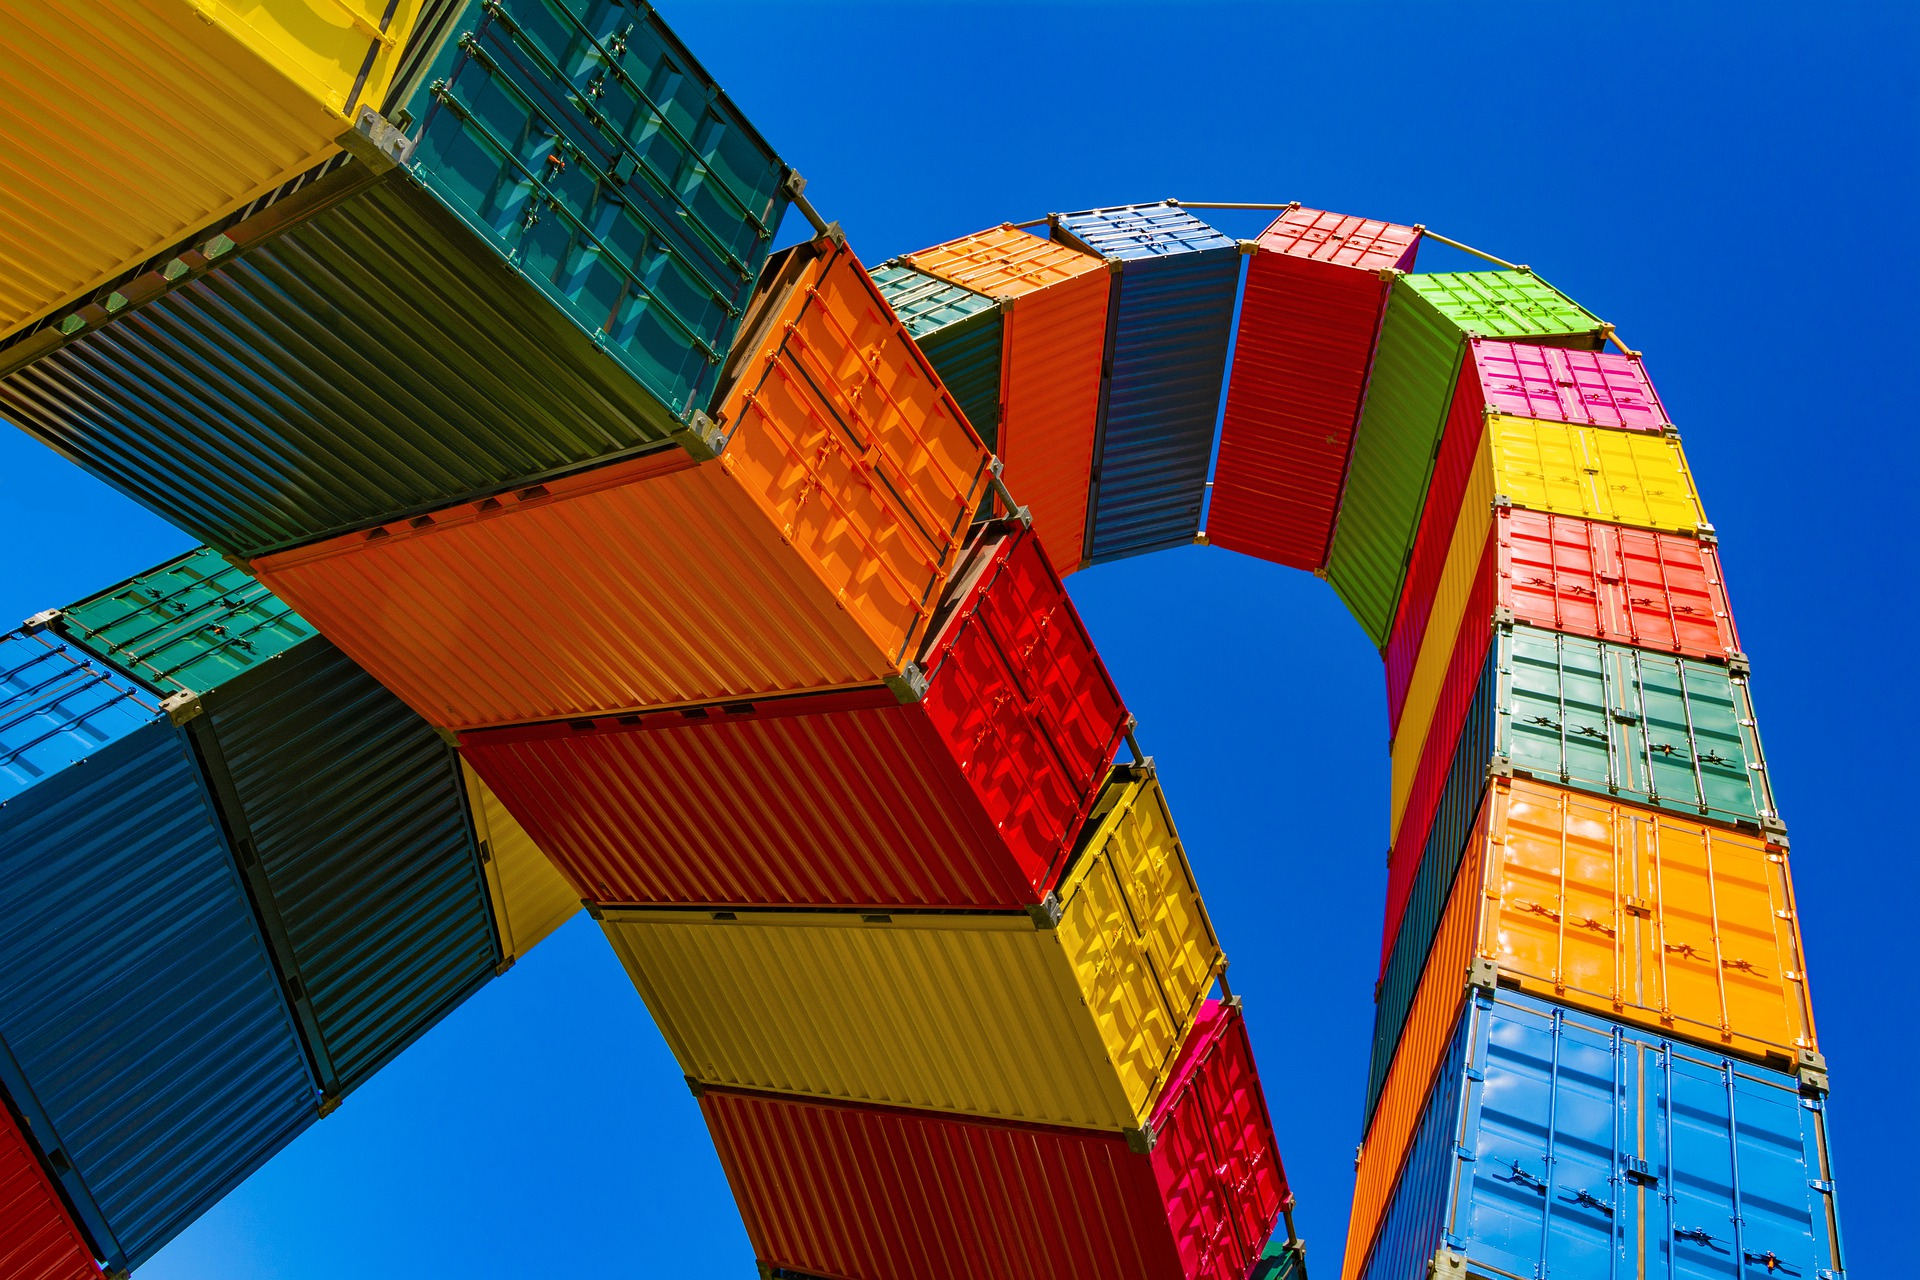
\includegraphics[scale=0.85]{images/container-4203677_1920.jpg}

\justify{}
Containerization is the process of encapsulating the code and dependencies for part or all of a project. The most popular
and common tool for realizing containerization is Docker\index{Docker}. Using Docker, we can programatically build an
environment for our project, and pass the entirety of this encapsulated environment from our local
development machine, into the Continuous Integration (CI)\index{Continuous Integration} pipeline for testing, and eventually
into our production environment. Containerization\index{containerization} helps us by offering a consistent operating
experience across disparate environments.

\justify{}
Recall our earlier discussion on the topics of immutability\index{immutability} and ephemerality\index{ephemerality}. It is more desirable
to create projects that are built and replaced frequently, than it is to attempt to upgrade and repair the infrastructure, 
platforms, and project code on an on-going basis. Attempts to patch and upgrade project hosts ``in place'', quickly reveal
great difficulty in maintaining consistency with the project source, even when that source is stored in a revision control system. 
These "in-place" upgrades and repairs may be the only option when it comes to certain software on ``bare metal'' hosts, and
hosts using certain virtualization technologies. A lesser degree of immutability
and ephemerality\index{ephemerality} also introduces issues keeping
operating system packages current, yet still compatible with the project. Imagine a situation where an upgrade to a package
is necessary to meet security requirements. What happens when this very same
upgrade means the project stops working since the package features that your application depends on have also changed?
The result is most likely angry end users and customers. Certainly not a situation we ever like to find ourselves in.

\section{Docker Conatiners}

\justify{}
Docker images are ``canned'' (as in, prefabricated) or custom directives for provisioning a Docker container. One or more
images can be used as building blocks when configuring our containers. For example, a Linux image and Python image might
be combined with our customizations that describe and point to our application code, all of which make up a single container
that provides the functions of a fully provisioned server. We get the added
benefit of being able to switch quickly between base operating system images with just a few lines of code change to our
project. For example, we could easily modify our container image to be predicated on Debian
rather than Red Hat distribution of Linux kernel and operating system should the need arise.

\section{Docker Hub}

\justify{}
This is a repository for Docker containers. Many pre-built container images are available for download
from \href{https://hub.docker.com/}{Docker Hub}. You can also create an account and upload your own images from your various
projects.

\section{What is a Dockerfile?}

\justify{}
The specification that outlines how a docker image is to be built is saved in the ``Dockerfile''.
The Dockerfile is our basic unit of containerization. That is to say,
our containers, and the applications they contain, are defined by the
Dockerfile. This Dockerfile will dictate how we provision resources and
include operating system essentials and packages inside our container.
Each Dockerfile is predicated on a base image, such as ``python:slim-buster''
for example.

\justify{}
One common technique to speed up our build pipelines is to simply pass along the Dockfile, rather than
building and passing a container image along to others.

\justify{}
\begin{mybox}{\thetcbcounter: Dockerfile}
  \lstinputlisting{code/04-docker/Dockerfile}
\end{mybox}

\justify{}
A valid Dockerfile begins with the \textbf{FROM} instruction. This instruction specifies the base image that we
will use to build our project on. These base images come from the
\href{https://docs.docker.com/docker-hub/repos/}{Docker Hub repositories}. We are setting an environment variable
\textbf{DEBIAN\_FRONTEND} to the value of noninteractive, which will cause the apt command to skip or ignore any
interactive menus that are encountered during execution of the apt command, since these would cause
our builds to ``hang up'' at an inaccessible interactive prompt. The \textbf{ADD} and \textbf{WORKDIR} directives
are meant to cause Docker to use the /workdir directory as the root of the project ``inside'' the
container. Finally, we are directing Docker to \textbf{RUN} and apt update and install the apt-utils package.

\section{Volumes}

\section{docker-compose.yml}
\justify{}
The docker-compose tool and its associated docker-compose.yml file allows us to manage multiple Docker containers for
one or more applications in the same project. We will add this file to our project to illustrate it's
composition and give ourselves the ability to extend our work later, as needed.

\justify{}
A file called docker-compose.yml\index{docker-compose.yml} will exist
alongside our Dockerfile in our docker directory.

\begin{mybox}{\thetcbcounter: Example docker-compose.yml}
  \lstinputlisting{code/04-docker/docker-compose.yml}
\end{mybox}

\justify{}
The docker-compose.yml file begins with a version specification. It's important to note that the commands and structure
of docker-compose.yml can vary widely based on this version. While versions cannot be mixed, all version are valid with
respect to docker-compose itself. We specify a service named ``devsecops'', and assign a host and container name. Under
``volumes'' we are mounting the base of the project directory in the host
filesystem as ``/project'' in the container filesystem. The build
``directive'' tells docker-compose how to locate the Dockerfile we wish to use for the containers.

\justify{}
With Docker properly installed and an understanding of the necessary configuration files, we can now do a bit of testing.
See the figure\ref{dockerdirectory} for an illustration of how to lay out the project files in your local file system.

\begin{figure}[!htb]
  \centering
  
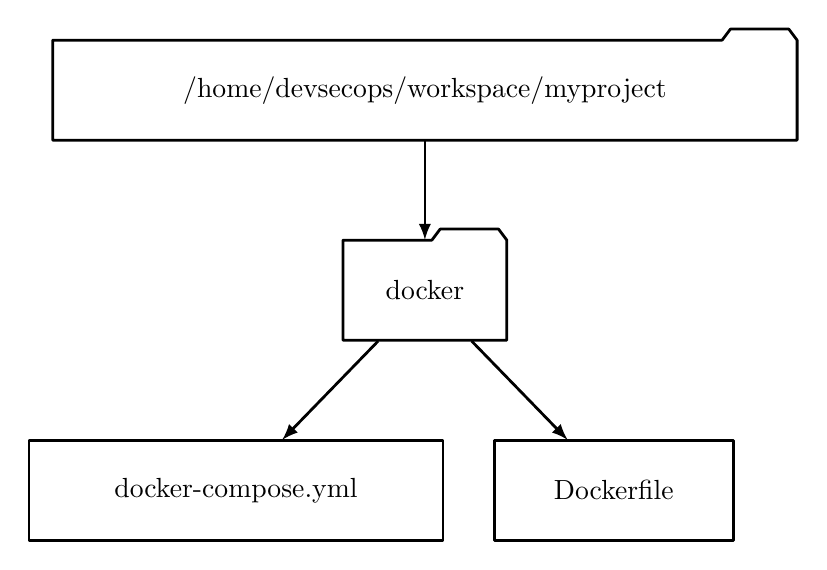
\begin{tikzpicture}[>=latex,line join=bevel,]
  \pgfsetlinewidth{1bp}
%%
\pgfsetcolor{black}
  % Edge: framework -> docker
  \draw [->] (142.5bp,143.7bp) .. controls (142.5bp,135.98bp) and (142.5bp,126.71bp)  .. (142.5bp,108.1bp);
  % Edge: docker -> dockercom
  \draw [->] (125.69bp,71.697bp) .. controls (117.37bp,63.135bp) and (107.19bp,52.656bp)  .. (91.116bp,36.104bp);
  % Edge: docker -> Dockerfile
  \draw [->] (159.31bp,71.697bp) .. controls (167.63bp,63.135bp) and (177.81bp,52.656bp)  .. (193.88bp,36.104bp);
  % Node: framework
\begin{scope}
  \definecolor{strokecol}{rgb}{0.0,0.0,0.0};
  \pgfsetstrokecolor{strokecol}
  \draw (276.5bp,180.0bp) -- (273.5bp,184.0bp) -- (252.5bp,184.0bp) -- (249.5bp,180.0bp) -- (8.5bp,180.0bp) -- (8.5bp,144.0bp) -- (276.5bp,144.0bp) -- cycle;
  \draw (142.5bp,162.0bp) node {/home/devsecops/workspace/myproject};
\end{scope}
  % Node: docker
\begin{scope}
  \definecolor{strokecol}{rgb}{0.0,0.0,0.0};
  \pgfsetstrokecolor{strokecol}
  \draw (172.0bp,108.0bp) -- (169.0bp,112.0bp) -- (148.0bp,112.0bp) -- (145.0bp,108.0bp) -- (113.0bp,108.0bp) -- (113.0bp,72.0bp) -- (172.0bp,72.0bp) -- cycle;
  \draw (142.5bp,90.0bp) node {docker};
\end{scope}
  % Node: dockercom
\begin{scope}
  \definecolor{strokecol}{rgb}{0.0,0.0,0.0};
  \pgfsetstrokecolor{strokecol}
  \draw (149.0bp,36.0bp) -- (0.0bp,36.0bp) -- (0.0bp,0.0bp) -- (149.0bp,0.0bp) -- cycle;
  \draw (74.5bp,18.0bp) node {docker-compose.yml};
\end{scope}
  % Node: Dockerfile
\begin{scope}
  \definecolor{strokecol}{rgb}{0.0,0.0,0.0};
  \pgfsetstrokecolor{strokecol}
  \draw (253.5bp,36.0bp) -- (167.5bp,36.0bp) -- (167.5bp,0.0bp) -- (253.5bp,0.0bp) -- cycle;
  \draw (210.5bp,18.0bp) node {Dockerfile};
\end{scope}
%
\end{tikzpicture}


  \caption{Project Directory and Docker related files.}
\label{dockerdirectory}
\end{figure}

\markdownInput{../code/ch4/lab-4a.md}

\subsection{Testing from GitHub}
\justify{}
In later chapter we will explore how to ``clone'' a project repository from \href{github.com} and do our work directory
from there. It is a good practice to keep a Dockerfile at the top level of your GitHUb repository that can be used to
build and test your application.

\section{Security Scanning Our Containers}
The \href{https://github.com/aquasecurity/trivy}{trivy container scanner} bills itself
as ``A Simple and Comprehensive Vulnerability Scanner for Containers and other
Artifacts, Suitable for CI''.

% https://www.paloaltonetworks.com/cyberpedia/what-is-container-security

\section{Podman and Buildah}

\justify{}
Note that Podman\index{Podman} is an acceptable substitute for Docker.
Podman is an Open Source tool from the Open
Containers Initiative (OCI)\index{Open Containers Initiative
(OCI)}. The Podman\index{Podman} service is said to be capable
of being a drop-in replacement for Docker, although it only
runs on Linux hosts at the time of this writing. Podman gives
the user the ability to use traditional Docker commands,
without the need to run a daemon to do so\cite{podman}, as is
the case with Docker.

\justify{}
You can install Podman by 
\href{https://podman.io/getting-started/installation.html}{following the instructions}
at their website. Once Podman is installed properly you
should be able to alias docker=podman and use it as a
drop-in replacement for Docker and it's associated daemon.

\section{Container Orchestration}

\justify{}
An orchestrator for containers can be thought of as an engine which
allows for their provisioning, deployment, scaling, monitoring, load
balancing, and more. The Container Orchestrator manages the
lifecycle and visibility of a container at all stages.

\justify{}
Kubernetes\index{Kubernetes} is an example, perhaps even the penultimate example, of a Container Orchestrator\index{orchestration}.
Folks throughout the DevSecOps, Software and Security communities are using Kubernetes these days, and
with good reason. It's adoption as a means to manage and replicate containers, and scale the applications they contain,
has been nothing short of revolutionary. System administrators and developers can do more, better work. Granted, this comes at
the expense of introduction yet another framework to learn, and no small amount of complexity.

\justify{}
An orchestrator helps us achieve immutability, and scale to meet user demand quickly and easily by abstracting away
concerns that come with operating workloads in a bare metal or VM environment.

\justify{}
Kubernetes and other orchestrators are rapidly evolving. To ignore this
game-changing ecosystem is to be left behind in terms of technological
prowess. Learning about containers, pipelines, infrastructure, and
so on are the foundational elements you will want to become familiar
with in preparation for expanding your mindset into the greater
dimensionality that orchestration realizes.

\justify{}
Later we will look more closely at the sprawling and vibrant topic of Kubernetes. For this stage of our journey to DevSecOps
enlightenment, it is enough to know that orchestration exists and have a bit of familiarity with its purpose.

\section{Further Reading}
